\documentclass{standalone}
\usepackage{ tikz }
\usepackage{ xparse }
\usepackage{../../../macros}

\begin{document}
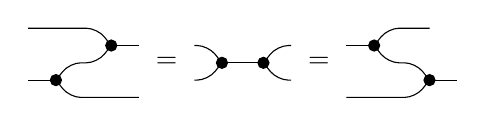
\begin{tikzpicture}[yscale=-1,x=1em,y=1.25em]
        
    \draw [rounded corners] (0,0) -- (2.5,0) -- (3,0.5);
    \draw [rounded corners] (0,1.5) -- (1,1.5);
    \filldraw (1,1.5) circle (2pt);
    \draw [rounded corners] (1,1.5) -- (1.5,1) -- (2.5,1) -- (3,0.5);
    \filldraw (3,0.5) circle (2pt);
    \draw (3,0.5) -- (4,0.5);
    \draw [rounded corners] (1,1.5) -- (1.5,2) -- (4,2);

    \node at (5,1) {$=$};

    \draw [rounded corners] (6,0.5) -- (6.5,0.5) -- (7,1);
    \draw [rounded corners] (6,1.5) -- (6.5,1.5) -- (7,1);
    \filldraw (7,1) circle (2pt);
    \draw (7,1) -- (8.5,1);
    \filldraw (8.5,1) circle (2pt);
    \draw [rounded corners] (8.5,1) -- (9,0.5) -- (9.5,0.5);
    \draw [rounded corners] (8.5,1) -- (9,1.5) -- (9.5,1.5);

    \node at (10.5,1) {$=$};

    \draw [rounded corners] (11.5,0.5) -- (12.5,0.5);
    \filldraw (12.5,0.5) circle (2pt);
    \draw [rounded corners] (12.5,0.5) -- (13,0) -- (14.5,0);
    \draw [rounded corners] (12.5,0.5) -- (13,1) -- (14,1) -- (14.5,1.5);
    \draw [rounded corners] (11.5,2) -- (14,2) -- (14.5,1.5);
    \filldraw (14.5,1.5) circle (2pt);
    \draw (14.5,1.5) -- (15.5,1.5);

\end{tikzpicture}
\end{document}